\documentclass[12pt,a4paper]{article}

% ------------------------------------------------
% Pacotes
% ------------------------------------------------
\usepackage[utf8]{inputenc}
\usepackage[T1]{fontenc}
\usepackage[brazil]{babel}
\usepackage{graphicx}
\usepackage[table]{xcolor}
\usepackage{array}
\usepackage{tabularx}
\usepackage{geometry}
\usepackage{fancyhdr}
\usepackage{mathptmx} % Times New Roman
\usepackage{enumitem}\usepackage{amsfonts}
\usepackage{amsmath} % Recomendado para o comando \text{}
\usepackage{amssymb}
\usepackage{tikz}
\usetikzlibrary{positioning, shapes.geometric}

% TikZ Styles for ER Diagrams
\tikzset{
    block/.style={rectangle, draw, thick, minimum width=2cm, minimum height=1cm, fill=white},
    diamond_node/.style={diamond, draw, thick, minimum width=2cm, minimum height=1cm, fill=white, aspect=2},
    attribute/.style={ellipse, draw, thin, minimum width=1.5cm, minimum height=0.6cm, fill=white, font=\scriptsize},
    line/.style={draw, thick},
}
% ------------------------------------------------ 
% Configuração de página
% ------------------------------------------------
\geometry{
    a4paper,
    left=2cm,
    right=2cm,
    top=2cm,
    bottom=2cm,
    headheight=15pt % Adicione isso
}% Caixa para resposta discursiva
\newcommand{\resposta}[1]{
\noindent
\framebox[\textwidth]{
\begin{minipage}{0.98\textwidth}
\vspace{#1}
\end{minipage}
}
}

\pagestyle{fancy}
\fancyhf{}
\renewcommand{\headrulewidth}{0pt}

\setlength{\parindent}{0pt}

% ------------------------------------------------
% Comandos auxiliares
% ------------------------------------------------
\newcolumntype{L}[1]{>{\raggedright\arraybackslash}p{#1}}
\newcolumntype{C}[1]{>{\centering\arraybackslash}p{#1}}

% ------------------------------------------------
% Documento
% ------------------------------------------------
\begin{document}

% ------------------------------------------------
% Cabeçalho - Corrigido para evitar aninhamento problemático
% ------------------------------------------------
\begin{tabularx}{\textwidth}{@{} L{4cm} X @{}}
    \raisebox{-0.5cm}{
\includegraphics[width=4cm]{Universidade_de_Rio_Verde.jpg}} &
    \hfill
    \begin{tabular}{|>{\centering\arraybackslash}m{10cm}|>{\raggedright\arraybackslash}p{1.8cm}|}
        \hline
        \cellcolor{black}\color{white}\rule{0pt}{1.2cm}\textbf{AVALIAÇÃO 1} 
        & 
        \scriptsize Nota \tabularnewline
        \hline
    \end{tabular} 
\end{tabularx}
\vspace{0.3cm}

% ------------------------------------------------  
% Tabela principal - Estrutura limpa
% ------------------------------------------------
\begin{tabularx}{\textwidth}{|X|L{2cm}|}
\hline
\textbf{Curso} & \textbf{Campus} \\
\textit{Engenharia de Software} & \textit{Rio Verde} \\
\hline
\multicolumn{2}{|l|}{\textbf{Disciplina}} \\  
\multicolumn{2}{|l|}{ \textit{Banco de dados}} \\
\hline
\textbf{Nome do(a) acadêmico(a)} & \textbf{Valor} \\
& 7,0 \\
\hline
\textbf{Professor} & \textbf{Turma} \\
\textit{ Sergio Souza Novak} & \textit{B} \\
\hline
\textbf{Data da Avaliação} & \textbf{Código} \\
\textit{19/03/2026} & \textit{ESW417} \\
\hline
\end{tabularx}
 
% ------------------------------------------------
% Barra de Atenção
% ------------------------------------------------
\vspace{0.2cm}

\begin{tabularx}{\textwidth}{|X|}
\hline
\cellcolor{black}\color{white}
\centering \textbf{ATENÇÃO:} Somente serão passíveis de \textbf{REVISÃO} avaliações resolvidas à \textbf{TINTA}. \tabularnewline
\hline
\end{tabularx}

\vspace{0.3cm}

\textbf{ORIENTAÇÕES PARA A RESOLUÇÃO}  

\begin{itemize}
    \item A avaliação é individual, sem consulta;
    \item A interpretação de texto faz parte da avaliação;
\end{itemize}

\vspace{0.5cm}

\begin{center}
    \rule{\textwidth}{0.4pt}
    \textbf{QUESTÕES}
\end{center}

\vspace{0.5cm} 

\begin{enumerate}
    \item A correta alocação da Chave Estrangeira (FK) é fundamental para evitar a redundância de dados e o excesso de valores nulos (NULL). Com base nas definições de mapeamento lógico e físico (SQL), responda o que se pede. Uma biblioteca possui Livros e Editoras. Uma editora pode publicar vários livros, mas cada livro é publicado por apenas uma única editora. Assinale onde a FK deve ser inserida:
    \begin{enumerate}[label=\Alph*)]
        \item A FK deve ser inserida na tabela \textbf{Editora}, pois é a entidade "forte".
        \item A FK deve ser inserida na tabela \textbf{Livro}, referenciando a Chave Primária de Editora.
        \item Deve-se criar uma terceira tabela para armazenar o relacionamento, por ser N:N.
        \item Ambos recebem FK um do outro para garantir a integridade.
        \item Não é necessário o uso de FK neste cenário.
    \end{enumerate}

    \item \textbf{Implementação SQL:} Com base no diagrama lógico abaixo, que representa a tabela \textbf{MEDICO} em um mapeamento de especialização/generalização (Tabela Única), assinale a alternativa que apresenta o código SQL (\texttt{CREATE TABLE}) \textbf{correto} para criar esta tabela. Utilize um campo \textbf{id} como Chave Primária (SERIAL) e garanta que o campo \textbf{crm} seja único (UNIQUE). Apenas o campo especialidade pode ser nulo.

    \begin{center}
    \begin{tikzpicture}[node distance=0cm, outer sep=0pt, every node/.style={draw, rectangle, minimum height=0.7cm, font=\small, anchor=north west}]
        \node (header) [fill=gray!20, minimum width=11cm] at (0,0) {\textbf{Tab.: MEDICO}};
        
        \node (col1) [minimum width=2cm] at (0,-0.7cm) {id (PK)};
        \node (col2) [minimum width=3cm] at (2cm,-0.7cm) {crm (UNIQUE)};
        \node (col3) [minimum width=3cm] at (5cm,-0.7cm) {nome};
        \node (col4) [minimum width=3cm] at (8cm,-0.7cm) {especialidade};
        
        \node (r1c1) [minimum width=2cm] at (0,-1.4cm) {1};
        \node (r1c2) [minimum width=3cm] at (2cm,-1.4cm) {CRM-123};
        \node (r1c3) [minimum width=3cm] at (5cm,-1.4cm) {Dr. Arnaldo};
        \node (r1c4) [minimum width=3cm] at (8cm,-1.4cm) {Cardiologia};
        
        \node (r2c1) [minimum width=2cm] at (0,-2.1cm) {2};
        \node (r2c2) [minimum width=3cm] at (2cm,-2.1cm) {CRM-999};
        \node (r2c3) [minimum width=3cm] at (5cm,-2.1cm) {Dra. Beatriz};
        \node (r2c4) [minimum width=3cm, fill=yellow!10] at (8cm,-2.1cm) {NULL};
    \end{tikzpicture}
    \end{center}

    \begin{enumerate}[label=\Alph*)]
        \item \texttt{CREATE TABLE MEDICO (id INTEGER, crm TEXT, nome TEXT, especialidade TEXT);}
        \item \texttt{CREATE TABLE MEDICO (id SERIAL, crm UNIQUE, nome NOT NULL, especialidade NULL);}
        \item \texttt{INSERT INTO MEDICO (id, crm, nome, especialidade) VALUES (1, 'CRM-123', 'Dr. Arnaldo', 'Cardiologia');}
        \item \texttt{CREATE TABLE MEDICO (id SERIAL PRIMARY KEY, crm TEXT UNIQUE NOT NULL, nome TEXT NOT NULL, especialidade TEXT);}
        \item \texttt{CREATE TABLE MEDICO (id PRIMARY KEY, crm UNIQUE, nome, especialidade);}
    \end{enumerate}

    \item \textbf{Cenário de Escolar:} Um Aluno pode se matricular em várias Disciplinas, e uma disciplina pode ter vários alunos matriculados. Como este relacionamento é resolvido no modelo lógico?
    \begin{enumerate}[label=\Alph*)]
        \item Inserindo a FK de Aluno na tabela \textbf{Disciplina}.
        \item Inserindo a FK de Disciplina na tabela \textbf{Aluno}.
        \item Criando uma tabela associativa (ex: \textbf{Matricula}) que contém as FKs de ambas as tabelas originais.
        \item Mesclando as tabelas Aluno e Disciplina em uma só.
        \item Transformando uma das entidades em um atributo multivalorado da outra.
    \end{enumerate}

 \item Com base no comando de criação de tabela abaixo, assinale a alternativa que apresenta o comando SQL (\texttt{INSERT INTO}) \textbf{correto} para inserir um novo registro na tabela \textbf{peixes}.

\begin{verbatim}
CREATE TABLE peixes (
    id TEXT,
    area INTEGER,
    perimetro DOUBLE PRECISION,
    ecentricidade DOUBLE PRECISION,
    maior_eixo DOUBLE PRECISION,
    menor_eixo DOUBLE PRECISION,
    peso INTEGER,
    classe INTEGER,
    compactacao DOUBLE PRECISION,
    rmm DOUBLE PRECISION,
    centroid_x DOUBLE PRECISION,
    centroid_y DOUBLE PRECISION
);
\end{verbatim}

\begin{enumerate}[label=\Alph*)]
    \item \texttt{INSERT INTO peixes (id, area, peso) VALUES ('P1', 500, 10);}
    \item \texttt{INSERT peixes ( area, peso) VALUES ( 500, 10);}
    \item \texttt{ADD TO peixes ( area, peso) VALUES ( 500, 10);}
    \item \texttt{INSERT INTO peixes VALUES ('P1', 500, 10);}
    \item \texttt{INSERT INTO peixes ('P1', 500, 10);}
\end{enumerate}



\vspace{0.8cm}

 \item (ENADE 2021) Uma Organização Não Governamental (ONG), relacionada à causa animal, registra os pets (animais de estimação) amparados por ela, de acordo com o seguinte Diagrama Entidade Relacionamento (DER). 

\begin{center}
    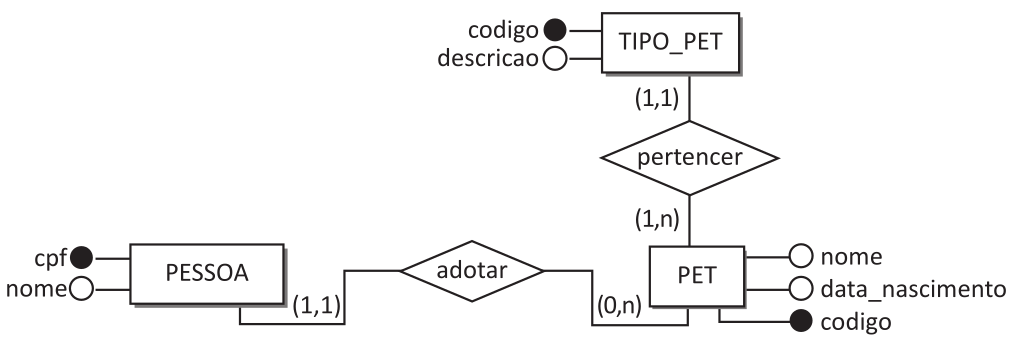
\includegraphics[width=0.8\textwidth]{diagrama1.png}
\end{center}

A partir das regras de mapeamento do Modelo Conceitual para o Modelo Lógico Relacional, assinale o Esquema Relacional mais adequado a ser gerado. Considere que as chaves primárias estão sublinhadas.

\begin{enumerate}[label=\Alph*)]
    \item \textbf{PESSOA}(\underline{cpf}: texto, nome: texto) \\
    \textbf{TIPO\_PET}(\underline{codigo}: inteiro, descricao: texto) \\
    \textbf{PET}(\underline{codigo}: inteiro, nome: texto, data\_nascimento: data, codigo\_tipo\_pet: inteiro, adotante: texto) \\
    \textit{codigo\_tipo\_pet referencia TIPO\_PET(codigo)} \\
    \textit{adotante referencia PESSOA(cpf)}
    
    \item \textbf{PET}(\underline{codigo}: inteiro, nome: texto, data\_nascimento: data) \\
    \textbf{PESSOA}(\underline{cpf}: texto, nome: texto, codigo\_pet: inteiro) \\
    \textit{codigo\_pet referencia PET(codigo)} \\
    \textbf{TIPO\_PET}(\underline{codigo}: inteiro, descricao: texto, codigo\_pet: inteiro) \\
    \textit{codigo\_pet referencia PET(codigo)}
    
    \item \textbf{TIPO\_PET}(\underline{codigo}: inteiro, descricao: texto) \\
    \textbf{PET}(\underline{codigo}: inteiro, nome: texto, data\_nascimento: data, codigo\_tipo\_pet: inteiro) \\
    \textit{codigo\_tipo\_pet referencia TIPO\_PET(codigo)} \\
    \textbf{PESSOA}(\underline{cpf}: texto, nome: texto, codigo\_pet: inteiro) \\
    \textit{codigo\_pet referencia PET(codigo)}
    
    \item \textbf{PET\_PESSOA}(\underline{codigo\_pet}: inteiro, nome\_pet: texto, data\_nascimento: data, \underline{cpf}: texto, nome\_pessoa: texto, codigo\_tipo\_pet: inteiro, descricao\_tipo\_pet: texto)
    
    \item \textbf{PESSOA}(\underline{cpf}: texto, nome: texto) \\
    \textbf{PET}(\underline{codigo}: inteiro, nome: texto, data\_nascimento: data, codigo\_tipo\_pet: inteiro, descricao\_tipo\_pet, adotante: texto) \\
    \textit{adotante referencia PESSOA(cpf)}
\end{enumerate}

\vspace{0.8cm}

 \item (ENADE 2014) Muitas aplicações utilizam o sistema de localização (GPS) do dispositivo móvel do usuário para descobrir qual o melhor caminho a seguir. Algumas aplicações também permitem que o usuário notifique a ocorrência de eventos que ele presencia durante seu percurso, tais como acidentes ou trânsito lento. Em um possível cenário, esta notificação é enviada para um servidor centralizado, o qual é responsável por disseminar a notificação para os demais usuários do aplicativo. Uma equipe de desenvolvimento criou uma aplicação desse tipo utilizando uma base de dados relacional para o armazenamento de dados referentes aos usuários, eventos e notificações enviadas. A modelagem conceitual foi feita utilizando o diagrama entidade-relacionamento conforme apresentado na figura a seguir.

\begin{center}
    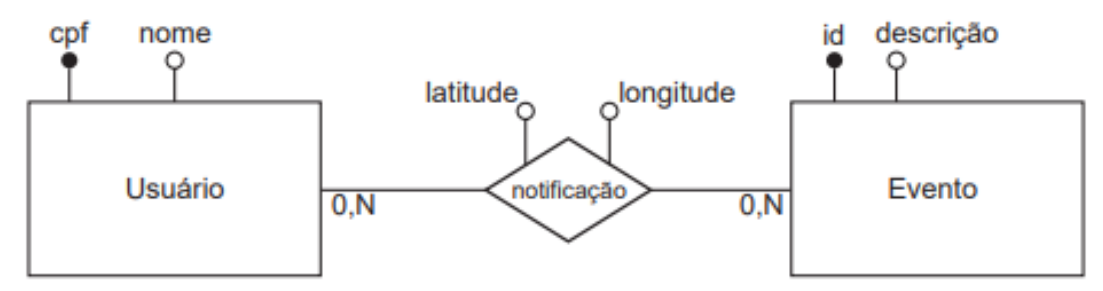
\includegraphics[width=0.8\textwidth]{diagrama2.png}
\end{center}

A equipe de desenvolvimento deseja adicionar as seguintes características ao modelo:
\begin{enumerate}[label=\roman*)]
    \item Cada notificação deve ter data e hora;
    \item O grupo de usuários para o qual uma notificação é enviada deve ser restrito. Cada usuário deve ter um grupo com um número arbitrário de amigos, que também são usuários da aplicação, e as notificações enviadas por um usuário devem ser enviadas somente a seus amigos. Também se deseja armazenar informações sobre quais notificações foram enviadas para quais usuários.
\end{enumerate}

Para atender a esses novos requisitos técnicos de modelagem, qual a alteração correta a ser feita?
\begin{enumerate}[label=\Alph*)]
    \item Adicionar atributos de data e hora na entidade \textbf{Notificação} e criar um relacionamento auto-relacionamento (N:N) em \textbf{Usuário} para representar "Amigo", além de uma entidade associativa entre Notificação e Usuário.
    \item Apenas adicionar data e hora na entidade \textbf{Evento}.
    \item Criar uma nova tabela para \textbf{GPS} e outra para \textbf{Celular}.
    \item Remover a entidade \textbf{Notificação} e usar apenas \textbf{Usuário}.
    \item Os requisitos já estão atendidos pelo diagrama original, nenhuma alteração é necessária.
\end{enumerate}

\vspace{0.8cm}

 \item (ENADE 2005)  Todo jogador deve pertencer a um único clube. Assinale a opção que representa corretamente, no modelo entidade-relacionamento, a especificação apresentada acima.

\begin{enumerate}[label=\Alph*)]
    \item \begin{tikzpicture}[baseline=(rel.base), node distance=1cm, every node/.style={scale=0.8}]
        \node[block] (clube) {clube};
        \node[diamond_node, right=of clube] (rel) {propriedade};
        \node[block, right=of rel] (jogador) {jogador};
        \draw[line] (clube) -- node[above] {(1,0)} node[below] {\scriptsize pertence a} (rel);
        \draw[line] (rel) -- node[above] {(n,0)} node[below] {\scriptsize possui} (jogador);
    \end{tikzpicture}
    
    \item \begin{tikzpicture}[baseline=(rel.base), node distance=1cm, every node/.style={scale=0.8}]
        \node[block] (clube) {clube};
        \node[diamond_node, right=of clube] (rel) {propriedade};
        \node[block, right=of rel] (jogador) {jogador};
        \draw[line] (clube) -- node[above] {(0,1)} node[below] {\scriptsize pertence a} (rel);
        \draw[line] (rel) -- node[above] {(0,n)} node[below] {\scriptsize possui} (jogador);
    \end{tikzpicture}
    
    \item \begin{tikzpicture}[baseline=(rel.base), node distance=1cm, every node/.style={scale=0.8}]
        \node[block] (clube) {clube};
        \node[diamond_node, right=of clube] (rel) {propriedade};
        \node[block, right=of rel] (jogador) {jogador};
        \draw[line] (clube) -- node[above] {(1,n)} node[below] {\scriptsize pertence a} (rel);
        \draw[line] (rel) -- node[above] {(0,n)} node[below] {\scriptsize possui} (jogador);
    \end{tikzpicture}
     
    \item \begin{tikzpicture}[baseline=(rel.base), node distance=1cm, every node/.style={scale=0.8}]
        \node[block] (clube) {clube};
        \node[diamond_node, right=of clube] (rel) {propriedade};
        \node[block, right=of rel] (jogador) {jogador};
        \draw[line] (clube) -- node[above] {(0,n)} node[below] {\scriptsize pertence a} (rel);
        \draw[line] (rel) -- node[above] {(0,n)} node[below] {\scriptsize possui} (jogador);
    \end{tikzpicture}
    
    \item \begin{tikzpicture}[baseline=(rel.base), node distance=1cm, every node/.style={scale=0.8}]
        \node[block] (clube) {clube};
        \node[diamond_node, right=of clube] (rel) {propriedade};
        \node[block, right=of rel] (jogador) {jogador};
        \draw[line] (clube) -- node[above] {(1,1)} node[below] {\scriptsize pertence a} (rel);
        \draw[line] (rel) -- node[above] {(0,n)} node[below] {\scriptsize possui} (jogador);
    \end{tikzpicture}
\end{enumerate}

\vspace{0.8cm}

 \item O diagrama a seguir apresenta um relacionamento ternário entre \textbf{Caminhão}, \textbf{Motorista} e \textbf{Pátio}. Assinale a alternativa que descreve a maneira correta de realizar a \textbf{eliminação do ternário} mantendo as mesmas regras de relacionamento entre as três entidades:

\begin{center}
\begin{tikzpicture}[node distance=2.5cm, every node/.style={scale=0.9}]
    % Entidades
     \node[block] (galpao) {Galpão};
    \node[block, below=of galpao] (patio) {Pátio};
    \node[block, left=of patio, xshift=-1cm] (motorista) {Motorista};
    \node[block, right=of patio, xshift=1cm] (caminhao) {Caminhão};


    
    \node[attribute, left=0.5cm of galpao] (gal_pk) {\underline{id\_gal}};
    \draw (galpao) -- (gal_pk);
    
    \node[attribute, left=0.5cm of patio] (pat_pk) {\underline{id\_pat}};
    \node[attribute, below left=0.5cm and 0.2cm of patio] (pat_nome) {nome};
    \draw (patio) -- (pat_pk);
    \draw (patio) -- (pat_nome);
    
    \node[attribute, above=0.5cm of motorista] (mot_pk) {\underline{id\_mot}};
    \node[attribute, above left=0.5cm and 0.5cm of motorista] (mot_nome) {nome};
    \draw (motorista) -- (mot_pk);
    \draw (motorista) -- (mot_nome);
    
    \node[attribute, above=0.5cm of caminhao] (cam_pk) {\underline{placa}};
    \node[attribute, above right=0.5cm and 0.5cm of caminhao] (cam_mod) {modelo};
    \draw (caminhao) -- (cam_pk);
    \draw (caminhao) -- (cam_mod);
    
    % Relacionamentos Binários
    \node[diamond_node, below=1cm of galpao, yshift=0.5cm] (rel_local) {localizado};
    
    % Relacionamento Ternário
    \node[diamond_node, below=1.5cm of patio] (rel_ternario) {escala};
    \draw[line, <-] (rel_ternario) -- ++(3,-3) node[left] {Relacionamento Ternário}; % Apontando para o ternário
    
    % Linhas e Cardinalidades
    \draw[line] (galpao) -- node[right] {(1,1)} (rel_local);
    \draw[line] (rel_local) -- node[right] {(1,n)} (patio);
    
    % Conexões do Ternário
    \draw[line] (patio) -- node[left] {(1,n)} (rel_ternario);
    \draw[line] (motorista) |- node[near start, left, yshift=0.5cm] {(1,n)} (rel_ternario);
    \draw[line] (caminhao) |- node[near start, right, yshift=0.5cm] {(1,n)} (rel_ternario);
     
\end{tikzpicture}
\end{center}

\begin{enumerate}[label=\Alph*)]
    \item Criar uma entidade associativa (ex: \textbf{Escala}) que possua relacionamentos binários (1:N) com as três entidades originais.
    \item Transformar o Pátio em um atributo do Motorista.
    \item Criar apenas um relacionamento binário entre Caminhão e Pátio ignorando o Motorista.
    \item Mesclar as três entidades em uma única tabela chamada "Logística".
    \item Relacionamentos ternários não podem ser eliminados ou convertidos no modelo de dados.
\end{enumerate}
\vspace{0.8cm}

 \item Com base no diagrama lógico abaixo, assinale a alternativa que representa o conceito de modelagem de dados utilizado para organizar as entidades \textbf{Animal}, \textbf{Vaca} e \textbf{Novilha}:

    \begin{center}
    \begin{tikzpicture}[node distance=1.2cm, every node/.style={draw, rectangle, minimum height=0.7cm, font=\small, fill=white}]
        % Superclasse
        \node (animal) [minimum width=3cm] {\textbf{Animal}};
        \node [below=0.1cm of animal, draw=none, fill=none, font=\tiny] {(Superclasse)};
        
        % Símbolo de especialização (Triângulo/Círculo comum em ER)
        \node (circ) [circle, draw, below=1cm of animal, xshift=0cm, inner sep=2pt] {S};
        \draw [line] (animal) -- (circ);
        
        % Subclasses
        \node (vaca) [below left=1.2cm and 0.5cm of circ, minimum width=2.5cm] {\textbf{Vaca}};
        \node (novilha) [below right=1.2cm and 0.5cm of circ, minimum width=2.5cm] {\textbf{Novilha}};
        
        \draw [line] (circ) -| (vaca);
        \draw [line] (circ) -| (novilha);
        
        % Atributos simples para ilustrar
        \node (id) [attribute, above left=0.5cm of animal] {\underline{id}};
        \draw (animal.north west) -- (id);
        
        \node (leite) [attribute, left=0.5cm of vaca] {producao\_leite};
        \draw (vaca) -- (leite);
        
        \node (idade) [attribute, right=0.5cm of novilha] {idade\_meses};
        \draw (novilha) -- (idade);
    \end{tikzpicture}
    \end{center}

    \begin{enumerate}[label=\alph*)]
        \item Polimorfismo.
        \item Encapsulamento.
        \item Especialização.
        \item Tautologia.
    \end{enumerate}

\end{enumerate}
\vspace{0.8cm}


\end{document} 